%!TeX program = xelatex
%!TeX encoding = utf-8
\documentclass{ctexart}
	\usepackage{fourier}
	\usepackage{amsmath}
	\usepackage{anysize}
	\usepackage[level]{datetime}
	\usepackage{lettrine}%首字下沉
	\usepackage{fontspec}
	\usepackage{tikz}%图形处理
	\usepackage{caption}%标记
	\usepackage{capt-of}%标记
	\usepackage[T1]{fontenc}
	\marginsize{2cm}{2cm}{2cm}{2cm}
	\newdateformat{ukdate}{\ordinaldate{\THEDAY} \monthname[\THEMONTH] \THEYEAR}%日月年
	\title{算法分析与设计作业}
	\author{陈斌 31617019}%陈斌  学号31617019
	\date{\ukdate\today}

	\begin{document}
		\maketitle
		\subsection*{}
			\textbf{6.3-3}
			\textnormal{证明: 对于任一包含$n$个元素的堆中,至多有 $\lceil\frac{n}{2^{h+1}}\rceil$ 个高度为$h$的结点?}
		\subsection*{解:}
			这里的高度为当前节点到叶子节点最长简单路径上的数目。我们已经知道从$\lfloor\frac{n}{2}\rfloor+1$到$n$的节点是叶子节点,也就是说最后一层的节点至多为$\lceil\frac{n}{2}\rceil$个。将$h=0$代入$\lceil\frac{n}{2^{h+1}}\rceil$中得$\lceil\frac{n}{2^{h+1}}\rceil = \lceil\frac{n}{2}\rceil$,所以在$h = 0$时成立。当$h = 1$时,我们把最后一层之上的节点看作是一个新的堆,此时新的堆的数量$n'=\lfloor\frac{n}{2}\rfloor$,新的堆的最后一层的节点至多为$\lceil\frac{n'}{2}\rceil = \lceil\frac{\lfloor\frac{n'}{2}\rfloor}{2}\rceil\leqslant\lceil\frac{n}{2^{1+1}}$,新的堆的最后一层的节点相当于原来的堆中高度为$1$的节点。以此类推当高度为$h$时,节点至多为$\lceil\frac{\lfloor\frac{n}{2}\rfloor}{2^h}\rceil\leqslant\lceil\frac{n}{2^{h+1}}\rceil$.
		\subsection*{}
			\textbf{6.4-1}
			\textnormal{参照图$6-4$的方法,说明$HEAPSORT$在数组$A = (4,13,2,25,7,17,20,8,4)$的操作过程。}
		\subsection*{解:}

			~\\
			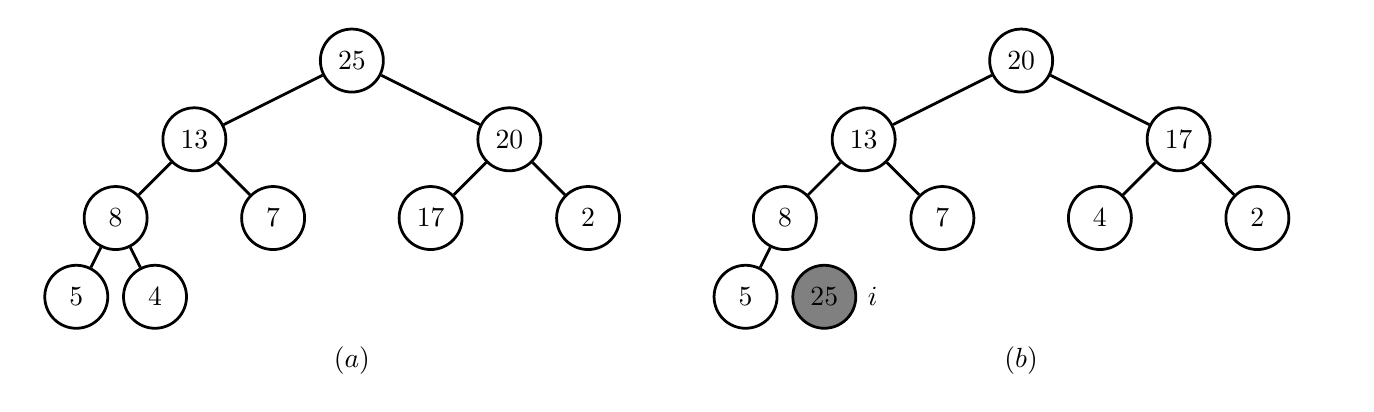
\begin{tikzpicture}[line width = 1pt,
								solid/.style = {circle, draw, fill = 
								gray, minimum size = 0.8cm},
								empty/.style = {circle, draw, fill = 
								white, minimum size = 0.8cm}]
						
				\node [empty] (a_1) at (4,4) {$25$};
				\node [empty] (a_2) at (2,3) {$13$};
				\node [empty] (a_3) at (6,3) {$20$};
				\node [empty] (a_4) at (1,2) {$8$};
				\node [empty] (a_5) at (3,2) {$7$};
				\node [empty] (a_6) at (5,2) {$17$};
				\node [empty] (a_7) at (7,2) {$2$};
				\node [empty] (a_8) at (0.5,1) {$5$};
				\node [empty] (a_9) at (1.5,1) {$4$};

				\draw (a_1) -- (a_2);
				\draw (a_1) -- (a_3);
				\draw (a_2) -- (a_4);
				\draw (a_2) -- (a_5);
				\draw (a_3) -- (a_6);
				\draw (a_3) -- (a_7);
				\draw (a_4) -- (a_8);
				\draw (a_4) -- (a_9); 
				\node [below=0.5cm, align=flush center,text width=8cm] at (4,1)
				{$(a)$};
				
					
				\node [empty] (a_1) at (12.5,4) {$20$};
				\node [empty] (a_2) at (10.5,3) {$13$};
				\node [empty] (a_3) at (14.5,3) {$17$};
				\node [empty] (a_4) at (9.5,2) {$8$};
				\node [empty] (a_5) at (11.5,2) {$7$};
				\node [empty] (a_6) at (13.5,2) {$4$};
				\node [empty] (a_7) at (15.5,2) {$2$};
				\node [empty] (a_8) at (9,1) {$5$};
				\node [solid, label = right:$i$] (a_9) at (10,1) {$25$};

				\draw (a_1) -- (a_2);
				\draw (a_1) -- (a_3);
				\draw (a_2) -- (a_4);
				\draw (a_2) -- (a_5);
				\draw (a_3) -- (a_6);
				\draw (a_3) -- (a_7);
				\draw (a_4) -- (a_8);
				\node [below=0.5cm, align=flush center,text width=8cm] at (12.5,1){$(b)$};
			\end{tikzpicture}

			~\\
			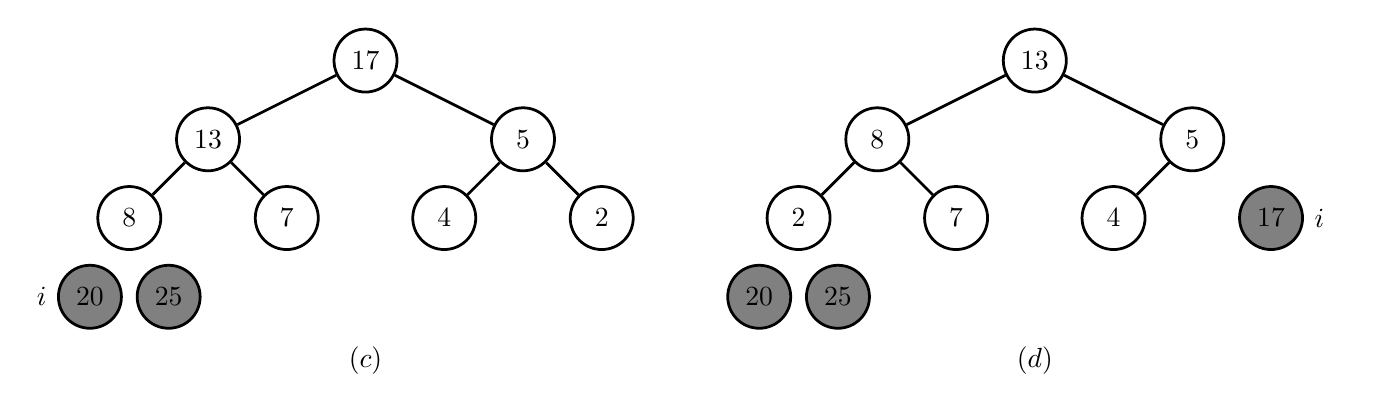
\begin{tikzpicture}[line width = 1pt,
								solid/.style = {circle, draw, fill = 
								gray, minimum size = 0.8cm},
								empty/.style = {circle, draw, fill = 
								white, minimum size = 0.8cm}]
						
				\node [empty] (a_1) at (4,4) {$17$};
				\node [empty] (a_2) at (2,3) {$13$};
				\node [empty] (a_3) at (6,3) {$5$};
				\node [empty] (a_4) at (1,2) {$8$};
				\node [empty] (a_5) at (3,2) {$7$};
				\node [empty] (a_6) at (5,2) {$4$};
				\node [empty] (a_7) at (7,2) {$2$};
				\node [solid, label = left:$i$] (a_8) at (0.5,1) {$20$};
				\node [solid] (a_9) at (1.5,1) {$25$};

				\draw (a_1) -- (a_2);
				\draw (a_1) -- (a_3);
				\draw (a_2) -- (a_4);
				\draw (a_2) -- (a_5);
				\draw (a_3) -- (a_6);
				\draw (a_3) -- (a_7);
				\node [below=0.5cm, align=flush center,text width=8cm] at (4,1)
				{$(c)$};
				
					
				\node [empty] (a_1) at (12.5,4) {$13$};
				\node [empty] (a_2) at (10.5,3) {$8$};
				\node [empty] (a_3) at (14.5,3) {$5$};
				\node [empty] (a_4) at (9.5,2) {$2$};
				\node [empty] (a_5) at (11.5,2) {$7$};
				\node [empty] (a_6) at (13.5,2) {$4$};
				\node [solid, label = right:$i$] (a_7) at (15.5,2) {$17$};
				\node [solid] (a_8) at (9,1) {$20$};
				\node [solid] (a_9) at (10,1) {$25$};

				\draw (a_1) -- (a_2);
				\draw (a_1) -- (a_3);
				\draw (a_2) -- (a_4);
				\draw (a_2) -- (a_5);
				\draw (a_3) -- (a_6);

				\node [below=0.5cm, align=flush center,text width=8cm] at (12.5,1){$(d)$};
			\end{tikzpicture}

			~\\
			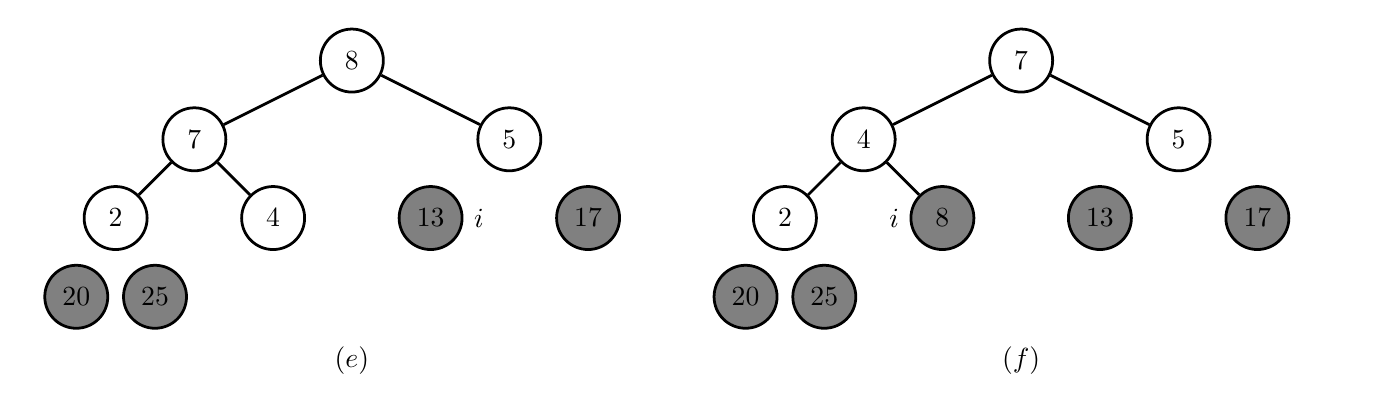
\begin{tikzpicture}[line width = 1pt,
								solid/.style = {circle, draw, fill = 
								gray, minimum size = 0.8cm},
								empty/.style = {circle, draw, fill = 
								white, minimum size = 0.8cm}]
						
				\node [empty] (a_1) at (4,4) {$8$};
				\node [empty] (a_2) at (2,3) {$7$};
				\node [empty] (a_3) at (6,3) {$5$};
				\node [empty] (a_4) at (1,2) {$2$};
				\node [empty] (a_5) at (3,2) {$4$};
				\node [solid, label = right:$i$] (a_6) at (5,2) {$13$};
				\node [solid] (a_7) at (7,2) {$17$};
				\node [solid] (a_8) at (0.5,1) {$20$};
				\node [solid] (a_9) at (1.5,1) {$25$};

				\draw (a_1) -- (a_2);
				\draw (a_1) -- (a_3);
				\draw (a_2) -- (a_4);
				\draw (a_2) -- (a_5);
				\node [below=0.5cm, align=flush center,text width=8cm] at (4,1)
				{$(e)$};
				
					
				\node [empty] (a_1) at (12.5,4) {$7$};
				\node [empty] (a_2) at (10.5,3) {$4$};
				\node [empty] (a_3) at (14.5,3) {$5$};
				\node [empty] (a_4) at (9.5,2) {$2$};
				\node [solid, label = left:$i$] (a_5) at (11.5,2) {$8$};
				\node [solid] (a_6) at (13.5,2) {$13$};
				\node [solid] (a_7) at (15.5,2) {$17$};
				\node [solid] (a_8) at (9,1) {$20$};
				\node [solid] (a_9) at (10,1) {$25$};

				\draw (a_1) -- (a_2);
				\draw (a_1) -- (a_3);
				\draw (a_2) -- (a_4);
				\draw (a_2) -- (a_5);

				\node [below=0.5cm, align=flush center,text width=8cm] at (12.5,1){$(f)$};
			\end{tikzpicture}
			
			~\\
			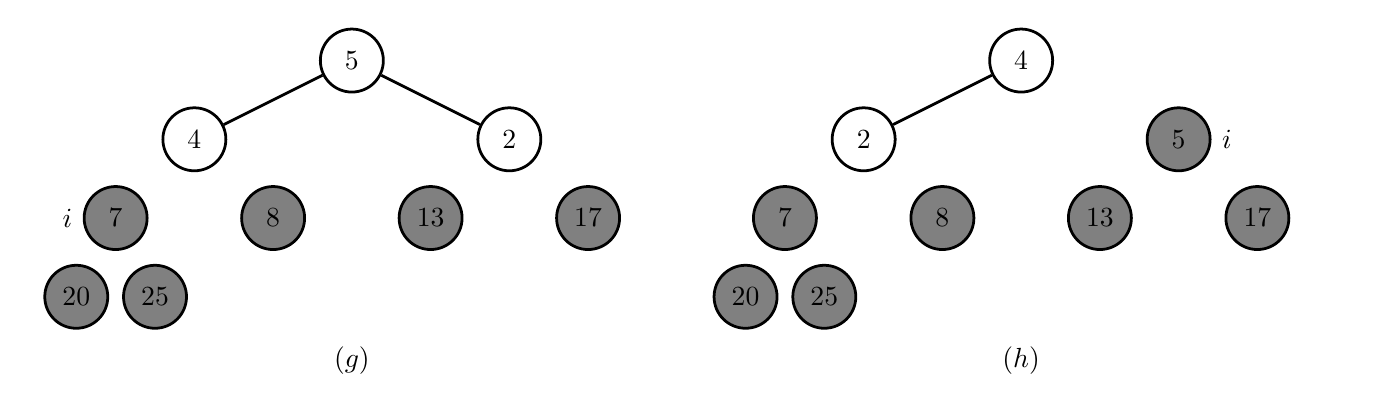
\begin{tikzpicture}[line width = 1pt,
								solid/.style = {circle, draw, fill = 
								gray, minimum size = 0.8cm},
								empty/.style = {circle, draw, fill = 
								white, minimum size = 0.8cm}]
						
				\node [empty] (a_1) at (4,4) {$5$};
				\node [empty] (a_2) at (2,3) {$4$};
				\node [empty] (a_3) at (6,3) {$2$};
				\node [solid, label = left:$i$] (a_4) at (1,2) {$7$};
				\node [solid] (a_5) at (3,2) {$8$};
				\node [solid] (a_6) at (5,2) {$13$};
				\node [solid] (a_7) at (7,2) {$17$};
				\node [solid] (a_8) at (0.5,1) {$20$};
				\node [solid] (a_9) at (1.5,1) {$25$};

				\draw (a_1) -- (a_2);
				\draw (a_1) -- (a_3);
				\node [below=0.5cm, align=flush center,text width=8cm] at (4,1)
				{$(g)$};
				
					
				\node [empty] (a_1) at (12.5,4) {$4$};
				\node [empty] (a_2) at (10.5,3) {$2$};
				\node [solid, label = right:$i$] (a_3) at (14.5,3) {$5$};
				\node [solid] (a_4) at (9.5,2) {$7$};
				\node [solid] (a_5) at (11.5,2) {$8$};
				\node [solid] (a_6) at (13.5,2) {$13$};
				\node [solid] (a_7) at (15.5,2) {$17$};
				\node [solid] (a_8) at (9,1) {$20$};
				\node [solid] (a_9) at (10,1) {$25$};

				\draw (a_1) -- (a_2);

				\node [below=0.5cm, align=flush center,text width=8cm] at (12.5,1){$(h)$};
			\end{tikzpicture}

			~\\
			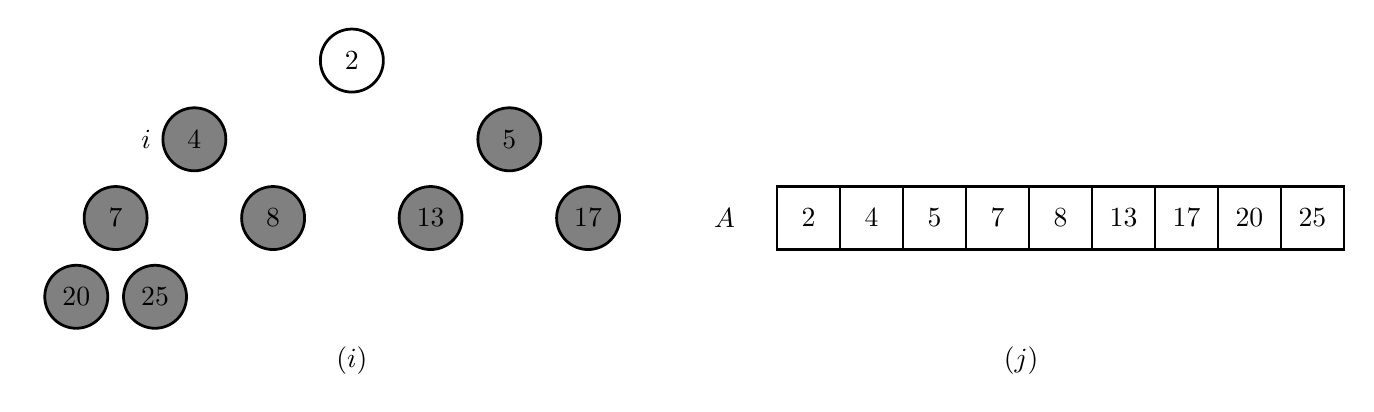
\begin{tikzpicture}[line width = 1pt,
								solid/.style = {circle, draw, fill = 
								gray, minimum size = 0.8cm},
								empty/.style = {circle, draw, fill = 
								white, minimum size = 0.8cm},
								rect/.style = {rectangle, draw, fill =
								white, minimum size = 0.8cm},
								]
						
				\node [empty] (a_1) at (4,4) {$2$};
				\node [solid, label = left:$i$] (a_2) at (2,3) {$4$};
				\node [solid] (a_3) at (6,3) {$5$};
				\node [solid] (a_4) at (1,2) {$7$};
				\node [solid] (a_5) at (3,2) {$8$};
				\node [solid] (a_6) at (5,2) {$13$};
				\node [solid] (a_7) at (7,2) {$17$};
				\node [solid] (a_8) at (0.5,1) {$20$};
				\node [solid] (a_9) at (1.5,1) {$25$};

				\node [below=0.5cm, align=flush center,text width=8cm] at (4,1)
				{$(i)$};
				
				\node [text width = 0.8cm] at (9,2) {$A$};
				\node [rect] (r_1) at (9.8,2) {$2$};
				\node [rect] (r_2) at (10.6,2) {$4$};
				\node [rect] (r_2) at (11.4,2) {$5$};
				\node [rect] (r_2) at (12.2,2) {$7$};
				\node [rect] (r_2) at (13,2) {$8$};	
				\node [rect] (r_2) at (13.8,2) {$13$};
				\node [rect] (r_2) at (14.6,2) {$17$};
				\node [rect] (r_2) at (15.4,2) {$20$};
				\node [rect] (r_2) at (16.2,2) {$25$};
				\node [below=0.5cm, align=flush center,text width=8cm] at (12.5,1)
				{$(j)$};
			\end{tikzpicture}
	\end{document}